\subsection{Context}

Conventional systems neuroscience experiments are typically short in duration
and often place significant constraints on subject behavior to simplify data
analysis.
%
However, these restrictions may limit our ability to observe critical
aspects of brain function and behavior that only manifest in more naturalistic
and extended conditions.

At the Sainsbury Wellcome Centre (SWC) for Neural Circuits and Behaviour, we
are pioneering Naturalistic, Long-Duration, and Continual (NaLoDuCo) foraging
experiments in mice that span weeks to months. During these extended
experiments, we collect high-resolution recordings of both behavioral and
neural activity in naturalistic settings.
%
In collaboration with the Gatsby Computational Neuroscience Unit (GCNU), we are
developing novel analytical methods to interpret this new class of data.

This novel experimental approach will enable researchers to explore neural
mechanisms underlying behavior over extended periods for the first time,
offering the possibility of uncovering insights across a wide range of
phenomena, including long-term behavioral adaptation, neural plasticity, and
learning.
%
The data generated from NaLoDuCo experiments represent an entirely
new resource in neuroscience, with the potential to drive breakthroughs and
discoveries that are beyond the reach of traditional experiments.

Our vision is to empower research centers worldwide to adopt this
groundbreaking approach.
%
However, the scale and complexity of the data generated pose significant
challenges in data acquisition, visualisation, and analysis.
%
In this proposal, we will address these challenges, developing and sharing
openly the necessary expertise, hardware, and software to enable this
transformative type of experimentation on a global scale.

\subsection{Focus areas and their challenges}

Below, we outline the key focus areas we aim to address
(Figure~\ref{fig:focusAreas}), along with their associated challenges.
%
These challenges primarily revolve around the collection and analysis of
continuously recorded, extremely large datasets--on the order of hundreds of
terabytes--gathered from experiments spanning weeks to months.

While experiments in neuroscience that are naturalistic, long-duration, or
continuous have been conducted in the past
\citep[e.g.,][]{jhuangEtAl10,maoEtAl21,volohEtAl23}, to the best of our
knowledge, we are the first to integrate all three of these features in a
single experimental paradigm.
%
This combination introduces unprecedented complexities in data processing, as
we aim to capture behavior and brain activity in their most ecologically valid,
extended, and uninterrupted forms.

\begin{figure}
    \begin{center}
        \resizebox{4.0in}{!}{%
            \resizebox{5in}{!}{%
    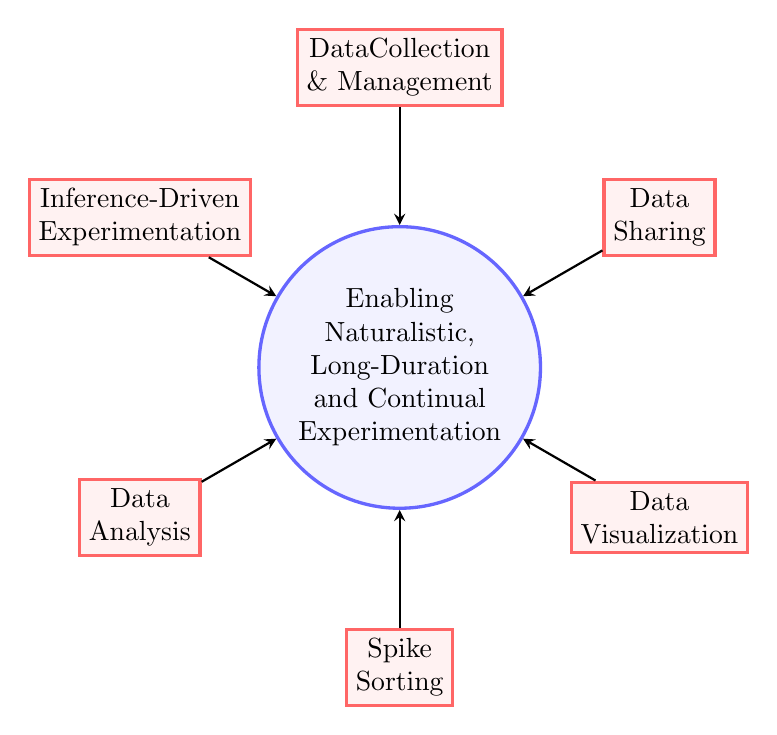
\begin{tikzpicture}[
            node distance=4cm and 1cm,
            centralNode/.style={circle, draw=blue!60, fill=blue!5, very thick,
            minimum size=7mm, align=center},
            itemNode/.style={rectangle, draw=red!60, fill=red!5, very thick,
            minimum size=5mm, align=center},
            arrow/.style={thick, <-, >=stealth},
        ]
        \node[centralNode] (naloducoExp)    {Enabling\\Naturalistic,\\Long-Duration\\and Continual\\Experimentation};
        % \node[itemNode]    (dataCol)        at (naloducoExp) ++(40:2cm) {DataCollection\\\& Management};
            \path (naloducoExp) ++(90:1.5in) node[itemNode] (dataCol) {DataCollection\\\& Management};
            \path (naloducoExp) ++(30:1.5in) node[itemNode] (dataSharing) {Data\\Sharing};
            \path (naloducoExp) ++(330:1.5in) node[itemNode] (dataVis) {Data\\Visualization};
            \path (naloducoExp) ++(270:1.5in) node[itemNode] (spikeSort) {Spike\\Sorting};
            \path (naloducoExp) ++(210:1.5in) node[itemNode] (dataAnalysis) {Data\\Analysis};
            \path (naloducoExp) ++(150:1.5in) node[itemNode] (inferenceDExp) {Inference-Driven\\Experimentation};
        \draw[arrow] (naloducoExp) -- (dataCol);
        \draw[arrow] (naloducoExp) -- (dataSharing);
        \draw[arrow] (naloducoExp) -- (dataVis);
        \draw[arrow] (naloducoExp) -- (spikeSort);
        \draw[arrow] (naloducoExp) -- (dataAnalysis);
        \draw[arrow] (naloducoExp) -- (inferenceDExp);
    \end{tikzpicture}
}

        }
    \end{center}
    \caption{Project theme (blue) and focus areas (red).}
    \label{fig:focusAreas}
\end{figure}

\subsubsection{Data acquisition and management}

At the SWC we have already performed foraging experiments in mice continuously collecting
behavioral and experimental data 24 hours a day for seven days.
%
We will share openly the specifications of the hardware used to build these
experiments (e.g., instructions for building large foraging arenas, video
cameras specifications, electrophysiological recording hardware), as well as
the software we used for experimental control, data quality control, data
access and management.

The data acquisition and management software used in our project is already
publically available in
GitHub\footnote{\url{https://github.com/SainsburyWellcomeCentre/aeon\_mecha}}.
%
This software is already being used by scientists at the Allen Institue for
Neural Dynamics and at Northwester University.
%
We will substantially improve its documentation to simplify its usage by
external users.

Challenges related to data acquisition and management include data indexing to
allow fast access to very large amount of saved data, online quality control
and alert systems to guarantee that anomalities in data collection are detected
and corrected with minimal delay, and syncrhonization between multiple data
streams.

\subsubsection{Data dissemination}

Datasets of the scale of hundreads of terabytes cannot be practically
downloaded from data repositories. This is specially true for contiguous
experiments where unique insights are extracted by characterizing full
datasets, and not only parts of them.
%
Therefore, we will store data in DANDI, which uses Amazon S3 buckets, and
provide software in Amazon EC2 instances to visualize and analyze data on the
cloud, avoiding costly data transfers.
%
That is, the large dataset sizes of NaLoDuCo experiments make it impractical to
distribute data to users and require to bring users to data.
%
Fortunately, cloud technologies are now mature to allows this.

Importantly, if we distributed these very large datasets to users, only those
in large research centers would have the computing power to process them. But, by deploying data
and computing in the cloud, any person with Internet access around the world
will be able to benefit from them.
%
Storing large datasets in DANDI is free.
% and it is possible to obtain cloud credits from Amazon to offer free compute to academic institution.

Dr.~Ben Ditcher, founder of CatalystNeuro, has played a pivotal role in
supporting the development and operations of the DANDI archive.

\subsubsection{Data visualisation}

Visualisations are essential for scientific discovery.
%
For the proposed project visualisation present two major challenges. First, they need
to display very large datasets at different temporal scales, from milliseconds
to weeks and months. Second, as data and software will be deployed in the
cloud, visualisation need to be web based.
%
Standard visualization tools cannot display terabyte sized datasets.
%
We will build custom web-based visualization tools to do this.

We have substantial experience building web-based visualization tools for
neurophysiological data. Dr.~Jeremy Magland is now developing
Neurosift\footnote{\url{https://github.com/flatironinstitute/neurosift}} a web-based
visualizer for DANDI datasets.

\subsubsection{Spike sorting}

When electrodes are placed in the brain, they typically record spikes from
multiple nearby neurons. Spike sorting attributes spikes to individual neurons.

Spike sorting is specially challenging for NaLoDuCo experiments.
%
First, because these experiments require to track individual neurons of freely
moving mice for weeks to months.
%
Second, because spike sorting needs to be done online, to allow experiments
driven by real-time machine learning inference, as described below.

Prof.~Sahani pioneered the use of Bayesian inference methods for spike
sorting~\citep{sahani99}.
%
Dr.~Jeremy Magland has significantly advanced the field of spike sorting,
particularly through his development of
MountainSort\footnote{\url{https://github.com/flatironinstitute/mountainsort5}}
and his contributions to
SpikeInterface\footnote{\url{https://github.com/spikeinterface/spikeinterface}}.

\subsubsection{Data analysis}

Advanced data analysis methods are indispensable to extract meaning from
NaLoDuCo experimental data.
%
However, analyzing this data is challenging for at least three reasons.
%
First, important insights will most probably come from the characterization of
complete datasets, and not form subsets extracted from them. Conventional batch
methods cannot be used with datasets of the size produced by NaLoDuCo
experiments.
%
For instance, for learning, batch linear regression cannot load into memory and
invert a data matrix with high-resolution observations from a one-month-long
experiment.
%
Thus, \textbf{online methods} that can process infinite data steams become
mandatory.

Second, a pervasive assumption in most ML algorithms is stationarity; i.e., the
assumption that the statistics of data do not change over time.
%
But in long-duration and continuous experiments this assumption is most often
violated as, for example, the arousal of subjects changes.
%
Hence, the analysis of data generated by these experiments requires
\textbf{adaptive methods}.

Third, statistical algorithms consist of two key stages: learning (or
trainning) and inference (or prediction). The learning stage identifies model
parameters, and the inference stage uses the learned model to make predictions,
or infer latent variables, from new unseen data.
%
Frequently training is performed on a small subset of a dataset, and inference
is done on the remaining data.  However, since in long-duration and continual
experiments behavior and neural activity are generall not stationary, it is not
optimal to train models on data subsets and use them to make inferences on the
remaining data, since the state of the animal at training and inference times
may be different.
%
To overcome this difficulty we will use \textbf{continual learning methods}.

We will evaluate methods to analyze different aspects of behavior and neural
activity (Figure~\ref{fig:dataAnalysisFocus}).
%
We will test how these methods process very large datasets, how they handle
non-stationary data, and how feasible is to retrain them to adapt to
changing conditions.
%
We will adapt these methods so that they better address these challenges and,
when needed, develop new ones.
%
We will carefully report the outcomes of these evaluations so that researchers
performing NaLoDuCo experimentation can choose the best methods that suit their
needs.

\subsubsection{Experiments driven by real-time machine learning inference}

Small animal experiments are usually controlled by simple static rules or
direct behavioral observations.
%
Funded by a BBSRC
award\footnote{\url{https://gow.bbsrc.ukri.org/grants/AwardDetails.aspx?FundingReference=BB\%2FW019132\%2F1}}
we are developing software to allow a new type of experimental control based on
statistical inferences made on behavioral and/or neural measurements.

For example, after inferring latent variables from neural activity and
observing that one of these latents have crossed a threshold, we can
deliver a reward \citep[as done in learning to control a
BCI;][]{clancyAndMrsicFlogel21}, or perform an action~\citep[as done in motor imagery
BCI;][]{lebedevAndNicolelis06}, or manipulate of neural activity~\citep[as
done when studying the causal relation between a pattern of brain activity and
behavior;][]{deisseroth15}.
%
We propose to further develop the previous software and use it to test causal
effects of neural activity patterns on foraging decisions using our NaLoDuCo
foraging experiments.

Buidling experiments driven by real-time machine learning inferences brings at
least two challenges. The first one is a machine learning problem, how to build
fast inferences that can operate in real time. The second one is a neuroscience
problem, how to identify neuroscience experiments suitable to real-time
control, and then perform the experiment with real-time control.
%
Fortunately at the Gatsby Unit we are experienced on building advanced machine
learning algorithms to address the first challenge. And at the SWC we perform
many sophisticated animal experiments that could benefit from real-time
experimental control.

In summary, we are pioneering a new paradigm in neuroscience experimentation,
driven by advanced inferential methods applied to rich behavioral and neural
recordings. This innovative technology has the potential to transform the
field, enabling experiments that were previously unimaginable. By leveraging
these sophisticated inferences, we may unlock new dimensions of knowledge that
could not be achieved through simpler, conventional approaches. This
breakthrough could open doors to insights that redefine our understanding of
brain-behavior relationships.


